\chapter{Introduction}\label{chap:introduction}
In past few years there has been a huge chatter about cloud computing. Every Organization in this era is at least reviewing or looking at resources to see if moving to cloud would same them time and efforts. Cloud as we are aware makes provisioning of new resources quickly so an organization can concentrate their efforts on tasks that create more value for them rather than concentrating their resources on procuring hardware or provisioning servers. At the same time companies do not want to invest in hardware that is hardly utilized for about 3-4 hours in a day thus making a classic case for moving to cloud. In cloud you utilize resources for the time you need and terminate the instance when your work is complete and paying only for the time a resource is up and utilized. 
\\

Businesses are often confused by the thought of moving to cloud. While they may have valid concerns, cloud supporters have advantages to show , but ultimately it is the business who has to decide if the advantages outweigh their concerns.\cite{MTechLabs}
\begin{figure}[!htb]
    \center{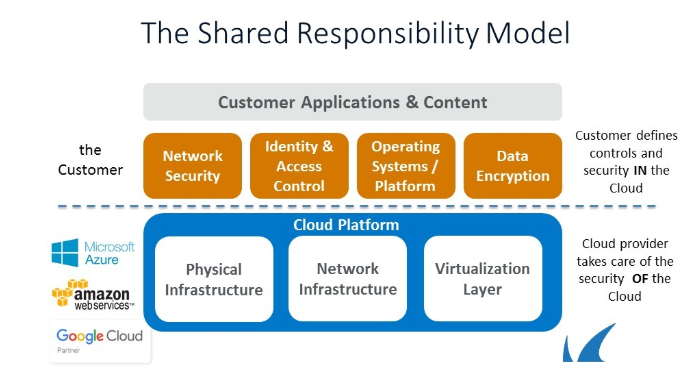
\includegraphics[width=\textwidth]
    {figures/experiments/Shared_Responsibility_Model.png}}
    \caption{\label{fig:shared_responsibility_model} Shared responsibility model}\cite{SecurityModel}
\end{figure}
%\begin{center}
%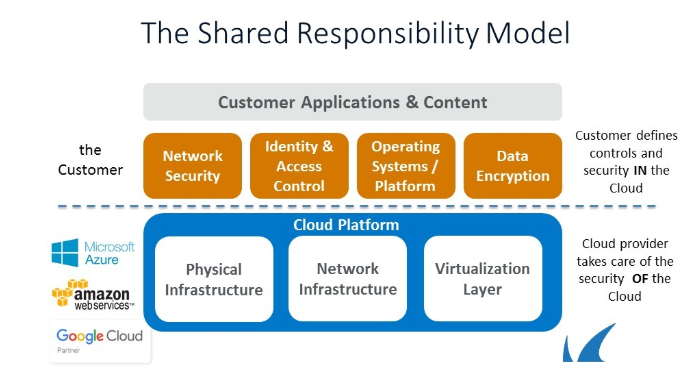
\includegraphics[scale=0.75]{figures/experiments/Shared_Responsibility_Model.png}
%\end{center}

\section{Concerns}
Concerns  and what do cloud supporters have to say about them : 


\subsection{Security}
Cloud environments experience – at a high level – the same threats as traditional data center environments, the threat picture is the same. Both run softwares, softwares have vulnerabilities, and there is someone out there waiting to exploit these vulnerabilities. However security on cloud is a shared responsibility model of security. While cloud provider takes care of the security of the cloud , some aspects of security remain sole responsibility of the consumer. Effective cloud security depends on knowing and meeting these consumer responsibilities. 

\subsection{Data Privacy} 
Cloud computing involves the dispersal of data across servers located anywhere in the world. Like globalization of networks. By crossing borders, involves considering countries with restrictive privacy and protection laws . This is somewhat covered as part of customer responsibility towards cloud security. For this corporations need to understand what kind of data will they load into cloud and who will have access to this data. \cite{DataPrivacy}

Other aspect of data privacy is handling sensitive data. Yes one of the problems is that this technology is light years ahead of the law and there are questions that need to be answered. Who owns the data, consumer or the hosting cloud provider? Can a cloud deny the consumer access to their own data or can it share this data with marketing firms  Obviously , the safest approach is data privacy is more a consumer responsibility. Keep data under proper control and apply data encryption methods. Regarding the question about laws, each company wants to protect their reputation. To get more clients and maintain them, cloud providers would uphold your data privacy. There are getting more managed and include all the necessary provisions that one should take while setting up their data on cloud. \cite{DataPrivacy2}

\subsection{ROI}
ROI or Return of Investment is widely a measure of financial success and can be a measured in a variety of ways. If you move to public cloud, you generally decrease invenstment but increase cost. With private cloud, it is vice-versa. But what matters is value to business, customer value, seller value, market brand value, corporate value. In case of cloud services, these relate to productivity, speed, size and quality. \cite{ROI}

\subsection{Implementation Cost}  

\subsection{Integration Issues} 
Most enterprises would apply an incremental model of implementation. It is less risky than big-bang. This requires integration of services.The risk of not being able to integrate is critical. If you cannot build a system, you cannot use it. This also adds to the cost of including glue-softwares to connect various interfaces .It could involve rewrite of code or existing process models. Not to forget significant skills are required to assemble and customize multiple cloud services , requiring the applications to be loosely coupled, programmed to perform in an integration layer instead of underlying infrastructure.  

\subsection{System Quality}  
\begin{itemize}
	\item Performance 
	\item Functionality 
	\item Manageability 
	\item User satisfaction 
\end{itemize}
